
% ===========================================================================
% Title:
% ---------------------------------------------------------------------------
% to create Type I fonts type "dvips -P cmz -t letter <filename>"
% ===========================================================================
\documentclass[11pt]{article}       %--- LATEX 2e base
\usepackage{latexsym}               %--- LATEX 2e base
%---------------- Wide format -----------------------------------------------
\textwidth=6in \textheight=9in \oddsidemargin=0.25in
\evensidemargin=0.25in \topmargin=-0.5in
%--------------- Def., Theorem, Proof, etc. ---------------------------------
\newtheorem{definition}{Definition}
\newtheorem{theorem}{Theorem}
\newtheorem{lemma}{Lemma}
\newtheorem{corollary}{Corollary}
\newtheorem{property}{Property}
\newtheorem{observation}{Observation}
\newtheorem{fact}{Fact}
\newenvironment{proof}           {\noindent{\bf Proof.} }%
                                 {\null\hfill$\Box$\par\medskip}
%--------------- Algorithm --------------------------------------------------
\newtheorem{algX}{Algorithm}
\newenvironment{algorithm}       {\begin{algX}\begin{em}}%
                                 {\par\noindent --- End of Algorithm ---
                                 \end{em}\end{algX}}
\newcommand{\step}[2]            {\begin{list}{}
                                  {  \setlength{\topsep}{0cm}
                                     \setlength{\partopsep}{0cm}
                                     \setlength{\leftmargin}{0.8cm}
                                     \setlength{\labelwidth}{0.7cm}
                                     \setlength{\labelsep}{0.1cm}    }
                                  \item[#1]#2    \end{list}}
                                 % usage: \begin{algorithm} \label{xyz}
                                 %        ... \step{(1)}{...} ...
                                 %        \end{algorithm}
%--------------- Figures ----------------------------------------------------
\usepackage{graphicx}

\newcommand{\includeFig}[3]      {\begin{figure}[htb] \begin{center}
                                 \includegraphics
                                 [width=4in,keepaspectratio] %comment this line to disable scaling
                                 {#2}\caption{\label{#1}#3} \end{center} \end{figure}}
                                 % usage: \includeFig{label}{file}{caption}


% ===========================================================================
\begin{document}
% ===========================================================================

% ############################################################################
% Title
% ############################################################################

\title{A parallel implementation of outlier detection over data streams}


% ############################################################################
% Author(s) (no blank lines !)
\author{
% ############################################################################
Kangqing YU\\
School of Computer Science\\
Carleton University\\
Ottawa, Canada K1S 5B6\\
{\em kangqingyu@cmail.carleton.ca}
% ############################################################################
} % end-authors
% ############################################################################

\maketitle

% ############################################################################
% Abstract
% ############################################################################
\begin{abstract}
Outlier detection has become an increasing challenging task in modern applications due to the fact that the data may come in the form of streams rather than statically as it was before. A lot of algorithms have been modified so that they can work in the streaming environment. Among all of them, a very popular technique called \textit{sliding window} is used, which only keep a portion of streaming data in memory and detect outliers purely based on those data. A main drawback with this approach is that the decision of outliers is only based on the data in current window and historical data are simply dropped and not considered in decision making of outlier data in current window. Therefore, this method fails to address the challenge of \textit{concerpt drift} in data streams. Another challenge in detecting outliers in data streams is that since the data may come at a very high rates and it is impossible to store all data in memory, the decision should be made in a timely manner with only one pass over data stream. This will pose a very harsh requirement in computational demends and in most case, it is impossible for CPU programming to achieve. In this project, I purposed a novel solution to detect outliers in streaming environment, powered by CUDA and MapReduce framework, based on a very efficient classical algorithm called LOF(Local Outlier Factor) to address the increasing challenge of outlier detection over continuous data streams. The proposed method, named C\_LOF is able to address the \textit{concerpt drift} in data streams, as well as detecting outliers in high-dimensional, high-rates data streams and produces timely results without compromising performances. Since the LOF algorithm is very computational expensive, very few works(almost none) have been conducted to extend the algorithm to work in streaming environment. As far as I know, the solution I purposed is the first algorithm that try to extend the LOF algorithm in the streaming environment and therefore it is also the first parallel implementation of LOF algorithm in the streaming context.
\end{abstract}


% ############################################################################
\section{Introduction} \label{intro}
% ############################################################################

An outlier in a dataset is a data point that is considerably different from the rest of the data as if it is generated by a different mechanism\cite{7516110}. Applications of outlier detections vary in numerous fields, including fraud detection, network intrusion detection, medical image screening, environment monitoring etc. A stream environment is where data come constantly at a high volume and may change over time. This can impose a very high requirement for computation power as decisions need to be made in real time within limited amount of time among all data. In addition to that, since the applications do not have random access to the underlying data in the streaming environment, when building an application that process data stream, these three key characteristics of data stream need to be taken into consideration: uncertainty, transiency, and incompleteness\cite{Sadik:2011:OOD:2076623.2076635}. Uncertainty means the data distribution of the model may change over the time as new data coming in a unpredictible way. This term is sometimes known as \textit{concept drift} in some literatures. Dealing with concept drift is a main challenge in most streaming applications. Transiency means it is not possible to store the entire dataset from data stream in the memory. The data can only be accessed in one pass and when it is processed, it should be deleted from memory. Completeness assume that the data will come indefinitely and they will never stop. These all make outlier detection in data streams extremely challenging from both algorithms and hardware perspective. 

To be more specific, suppose you have a data stream that keeps coming indefinitely, at one time $t_{i}$, you identify object $o_{k}$ as being outlierness in the current window. And after some time $W$ at time $t{i} + W$ when the whole recent history is considered, object $o_{k}$ may become an inliner.  And vice versa. This can be illustrate in Figure \ref{fig:evolving}

\includeFig{fig:evolving}{Figures/evolving-data}{Evolving 2D data stream}

In this project, I developed an novel, modified version of \textit{Local Outlier Factor} algorithm, called Cumulative Local Outlier Factor, or C\_LOF in short, with the support of statistical binned summary, where an outlier decision is considered not only based the data points in the current data window, but also taking consideration of historical data without the necessity storing the entire dataset in the secondary memory. In doing so, I kept a statistical binned summary of all the observed data to help making decisions on outlier for data points within current processing window, and gradually fade away the impact of the obsolete data when making decisions on current data. Thus the proposed algorithm should provide a more accurate results compared to the widely used sliding window approach. 

Note that most density-based approaches in outlier detection, including LOF, despite being accurate, are notorious of being computational expensive. And therefore, it is almost impossible to detect outliers with high volume, high speed data streams without introducing parallelism. Other computational in-expensive algorithms exists but they either need to sacrifice on the accuracy or assuming fixed distribution over the underlying data, which fails to capture the nature of \textit{concerpt drift} in data streams. To address the expensive computation demands of the LOF algorithms over data streams, I employed parallelism in this project as an implementation of the proposed algorithm. To be more specific, the C\_LOF algorithm is implemented on GPU with CUDA framework to accelerate the computational time in order to provide timely results over the high input rates of streaming data and the maintenance of binned summary is implemented using the MapReduce programming paradigm, which to a great extent, simplify the problem as well as leaving a lot of rooms for parallelizing. 

%\ref{proa} give a details explaination on the algorithm

The accuracy of the result produced by this algorithm is compared with \textit{sliding-window} based methods, where no historical data is considered to show whether it can help predict outliers more accurately, by mining historical data. In addition, the performance of the purposed C\_LOF algorithm under the GPU implementation is also measured against CPU implementation of LOF, where no parallelism is used to further illustrate if the proposed method can achieve a significant speedup for outlier detection compared with sequential implementation.

% ############################################################################
\section{Literature Review} \label{litrev}
% ############################################################################

A lot of techniques have been introduced in last decades to solve the outlier detection problem. And these techniques can be briefly summarized into three different categories: 

\begin{enumerate}
  \item Supervised approaches
  \item Semi-supervised approaches
  \item Unsupervised approaches
\end{enumerate}

Supervised approaches typically require building a prediction model for rare events based on manually labelled data(the training set), and use it to classify new event based on the learnt model\cite{Joshi:2001:MNH:376284.375673,sup02}. In other words, the outlier problem in this case becomes a classification problem where we are only interested in the minority class whose data deviate largely from the rest. The main problem with this approach is that in order to ensure accuracy, a large number of labelled data need to be generated which is unpractical in most cases.
 
Compared to supervised approaches, Semi-supervised approaches\cite{Basu:2004:PFS:1014052.1014062,semi-sup02} only require a small number of training data with some unlabeled data to obtain better predictions. One approach introduced by Jing Gao et al.\cite{Gao:2006:SOD:1141277.1141421} takes advantage of K-mean clustering in unsupervised learning by adding penalties to the objective function for mislabelled data points and optimize the overall objective function. 

Although some of those techniques may generate very promising results, they work well only in static data and typically don't fit into the context of dynamic streaming environment. In other words, both supervised and semi-supervised methods will assume that they will have \textit{random access} to the underlying data while this is not possible for streaming data when you can only have portion of it at one time and they also fails to address the problem of the potential change of data distribution.

In contrast, unsupervised learning methods don't require labelled input and typically don't assume a fixed data distribution as the model can be dynamically built based on variations of data. Many best-known techniques of outlier detection fall into this category and based on the context, they can mostly be classified into two categories: \textbf{Unsupervised outlier detection on static data} and \textbf{Unsupervised outlier detection on streaming data}. 

\textit{Distance-based approach} was among the very first outlier detection method introduced by Knorr and Ng\cite{EKnorr:1998} that detect outliers in a static environment. It calculates the pair-wise Euclidian Distance between all data and if one data point has less than $k$ neighbors within distance $R$, it is considered an outlier. There are some variants of the static distance-based approaches, and their ideas are quite similar. For instance, Ramaswamy et al.\cite{Ramaswamy:2000:EAM:342009.335437} purposed a method where an outlier is defined by considering the total number of objects whose distance to its $k^{th}$ nearest neighbor is smaller than itself. Angiulli and Pizzuti\cite{1377172} introduced a method where an outlier is defined by taking into account of the sum of the distances from $1^st$ up to the $k^{th}$ nearest neighbors. These methods are sometimes referred as KNN and it should be noted that it is different from the term KNN in supervised machine learning. 

\textit{Density-based approach} is another way to detect outlier on static data. The basic idea is to assign a degree of being outlier(a score) based on the density of local neighbourhood, given some predefined restrictions. A popular example of this approach is Local Outlier Factor(LOF) algorithm\cite{Breunig:2000:LID:342009.335388}, which is what this proposed algorithm is based on, use the concept called \textit{reachability} to coin the density of data point. The density of each data point is measured by considering the reachability of this data point, in regards to the reachabilities of its neighbors', as shown in Figure \ref{fig:lof}. Another popular density-based outlier detection method is called LOCI(Local Correlation Integral)\cite{1260802}

\includeFig{fig:lof}{Figures/lof}{The Local Outlier Factor (LOF) algorithm}

There are some other types of outlier detection techniques on static data. \textit{Statistics approach}, which is based on the probability theory and normally models the underlying data using a stochastic distribution(e.g. Gaussian distribution). One of the most popular one used is \textit{auto-regression} model or sometimes being referred as Gaussian mixture model\cite{4438332}; \textit{Deviation approach}, which is first introduced by Arning et al.\cite{A.Arning:deviation}, where an outlier is detected if feature space of one data point deviates largely from other data points; Another recent technique introduced by Harkins et al.\cite{S.Harkins:rnn} takes advantage of replicator neutral network(RNN) to detect outliers. There might be other techniques used for unsupervised outlier detection but due to the limitation of this paper, I can only list some of them. The ones mentioned above are those best-known so far to detect outliers statically.

%Aggarwal and YU\cite{Aggarwal:2001:ODH:375663.375668} proposed a technique for outlier detection. The basic idea in their definition is, a point is an outlier, if in some lower dimensional projection it is present in a local region of abnormally low density. This method is also an efficient method for high dimensional data set\cite{04666541}. 

As modern applications have an increasing demands to process streaming data in real-time, a lot of these static methods mentioned before have been extended to work in the dynamic streaming environments. The all based on the same ideas in static approaches but algorithms have been modified in an incremental fashion to address the \textit{concept drift} of the data stream properties.

Distance-based outlier detection approach was among the first which start to apply the method in the streaming context. In the last decade, there are several studies which focus on \textit{distance-based outlier detection in data streams(DODDS)}. Due to the fact that the distance-based require random access on the data and this is not possible with stream data, \textit{sliding window} technique was introduced which only keep a number of active objects in current window. When objects expire, they are deleted from memory as new object comes in. There are mainly two window models in data streams: count-based window and time-based window

Numerous algorithms have been invented to process stream data using sliding window on outlier detection. And based on the benchmark among all DODDS algorithms given by Luan Tran et al.\cite{Tran:2016:DOD:2994509.2994526}, the MCOD algorithm introduced by M.Kontaki et al.\cite{5767923} seems to have the most satisfying performance. Its basic idea is to pre-compute the \textit{safe inliers} that have more than $k$ neighbors which arrived after $p_{i}$ by using an event queue, which can reduce greatly on space complexity. Because the neighbors which arrives before $p_{i}$ may expire, by declaring the neighbors which arrived after $p_{i}$ to be larger than $k$, we can safely mark $p_{i}$ as inlier. The time complexity of this algorithm is guaranteed to be $O(n\log{k})$ while maintaining the space complexity to be $O(nk)$

Most of DODDS algorithms are based on the original definition of distance-based technique given by Knorr and Ng\cite{EKnorr:1998}. The other distance-based techniques in outlier detection such as KNN remain unsolved in the streaming context. It would be interested to see if those methods can be extended to work in the data streaming context. Since all DODDS methods only have access to only a portion of data, they all lack a global view of the entire dataset and in most cases, there accuracies are not guaranteed. 

\textit{Clustering} is another technique to outlier detection on stream data. Since clustering is a technique in unsupervised machine learning, it inspired the ideas of outlier detection in streaming environment. Two main algorithms exists for clustering-based approaches. One of them is called \textit{K-Mean clustering}\cite{04666541}, which also use the idea of sliding window and cluster the data in each window. But different than the distance based approach, the detected outliers are not reported immediately but rather be considered as a \textit{candidate outlier}. A metric which measure the mean value of each clusters is maintained and carried over to next window in stream to further compare with data in other chunks. If the candidate outlier passed a given number of windows, it is then identified as \textit{real outlier}. Compared to K-Mean clustering, \textit{K-Median clustering}\cite{DBLP:journals/corr/abs-1002-4003} clusters each chunk of data into variable number of clusters(from $k$ to $k log(n)$), and it passes the weighted medians found in current window into next one for testing outlierness rather than the mean and candidate outliers. Both of these two approaches will require users' input of value $k$ but K-Median clustering theoretically is better since the number of clusters is not fixed. 

To address this problem of storage and users' input parameters, an ideal method need to find a efficient way to efficiently mine its historical data or gradually fade old data away without users' intervention. An technique inspired from \textit{sensor network} is mentioned in\cite{Subramaniam:2006:OOD:1182635.1164145}, where it use a \textit{kernel density estimator} to model the distribution of the sensor data. When used for outlier detection, the number of neighbors of a given data point $p_{i}$ is estimated by the distribution function $f(p_{i})$. In \cite{4221341}, D. Pokrajac et al illustrated that the LOF algorithm can be applied incrementally and the insertion of new data as well as deletion of obsolete data does not depend on the total number of $N$ in dataset and therefore the time complexity of incremental LOF algorithm can theoretically be $O(N\log{N})$. These two methods are both based on computing of the densities of local neighbourhood. However, there are still a lot of noise around these algorithms and many researchers argue that it is still computational expensive in practice. Also the LOF approach proposed by D. Pokrajac et al will need to store the entire dataset, which is not applicable in the streaming context.

Even though there are many studies in the last decade that focusing on detecting outlier online in data stream, only a few tried to solve this problem using a parallel implementation. In \cite{7516110} C. HewaNadungodage et al.implemented a so-called SOD\_GPU\footnote{Stream Outlier Detector-GPU} algorithm which is based on kernel density estimator powered by GPU to effectively detect outlier in continuous data streams. The results seems very promising as it is 20X faster compared to a multicore CPU implementation and even a higher accuracy rate compared to the sliding window approach. And this is the only work, I found by the time of writing, which tried to solve the outlier detection problem in streaming environment using parallel computing approach. Other parallel implementations for outlier detection exist but they only work in a static fashion, in which case, it does not seem to be quite necessary. In \cite{6641405},  Angiulli et al. proposed a distance-based KNN algorithm powered by GPU and similarly, Matsumoto and Hung\cite{Matsumoto2012} introduced a GPU-accelerated approach to detect the outliers in uncertain data. Another GPU-accelerated approach to detect outlier in static data was purposed in \cite{Alshawabkeh:2010:ALO:1735688.1735707}, where the LOF(Local outlier factor) algorithm is used. Anna Koufakou et all.\cite{4634266} developed a parallel outlier detection strategy based on \textit{Attribute Value Frequency(AVF)}\cite{4410382}\footnote{Note that the AVF algorithm can only detect outlier in categorical data.} algorithm using MapReduce programming paradigm. Other incremental parallel methods exist for online outlier detection but they either require storing the entire history of data stream or giving a set of user-defined parameters, which is hard to define in most cases. 

% ############################################################################
\section{Proposed Approach} \label{proapp}
% ############################################################################

Unlike the classical LOF algorithm, the proposed C\_LOF method is capable of processing outlier in data stream $S = {X_1, X_2, X_3, ......., Xn, .......}$ without storing all observed data, where each data point $S_i$ can be arbitrary dimension of $d$ e.g. $X_i = <x_{i1}, x_{i2}, ......., x_{id}>$. This is achieved by keeping a binned summary of all processed data and these summary statistics is used to help decide the Local Outlier Factor of future data points. Specifically, the binned summary acts as \textit{virtual data points}, whose \textit{local reachability density(lrd)}(explained later) is pre-calculated based on the frequencies of previous data that fall into that bin, and do not need to calculate the LOF values of their own. The full details of this algorithm is explained in following:

% ----------------------------------------------------------------------------
\subsection{Local Outlier Factor} \label{subsect1}
% ----------------------------------------------------------------------------

The main idea of LOF algorithm is to assign each data point a degree(score) of being outlier. And this degree(score) is called \textit{Local Outlier Factor(LOF)} of this data point. This metrics measure the density of a data point compared with its neighbourhood(K-nearest neighbors). The computing of LOFs for all data points typically comprise of following steps\cite{Breunig:2000:LID:342009.335388}:

\begin{enumerate} \label{lof_algorithm}
	\item For each data point p, compute its \textbf{k-distance(p)} as distance to its k-th nearest neighbor of p
	\item For each data point p, find its \textbf{k-distance-neighbourhood} of p, which contains every object $o$ whose distance to p, noted as $d(o, p)$ is not greater than \textbf{k-distance(p)}
	\item For each data point q in the \textbf{k-distance-neighbourhood} of p, calculate its reachability distance with respect to data record p as follows:
		\begin{equation} \label{rdist}
			\textbf{reach-distk(p,q)} = max(d(p,q), k-distance(q))
		\end{equation}
	\item For each data point p, calculate its \textbf{local reachability density(lrd)} of q as inverse of the average reachability distance over k-nearest neighbor of p:
		\begin{equation} \label{lrd}
			\textbf{lrd(p)} =  \frac{1}{\sum\limits_{k \in knn(p)} reach-distk(p,q) / k}
		\end{equation}
	\item And finally, for each data point p, calcuate its \textbf{LOF} as ratio of average \textbf{lrd} over k-nearest neighbor of p and \textbf{lrd} of p it self
		\begin{equation} \label{lof}
			\textbf{LOF(p)} = \frac{\frac{1}{k} \sum_{k \in knn(p)} lrd(p)}{lrd(p)}
		\end{equation}
\end{enumerate}

The outlierness is detected once the difference between the LOF value of data point p and the average value of LOF over all observed data is greater than a pre-defined hyper-parameter $\theta$. Based on my experiments, the value of $\theta$ should be something between $[0.2, 0.5]$ and if the LOF value of a data point is greater than 1, this will highly likely to be a outlier.

To extend the LOF algorithm in context of data stream, I borrowed the idea of \textit{sliding window} from DODDS(distance-based outlier detection in data stream) and maintain chunks of data points in memory. But different from DODDS which take no consideration of historical data, I apply the LOF algorithm over data points in current window plus the virtual data points from the binned statistical summary(explained shortly). This will give a more accurate estimate of outliers since some synopsis of previous data points is maintained.

% ----------------------------------------------------------------------------
\subsection{Maintaining Binned Statistical Summary} \label{subsect2}
% ----------------------------------------------------------------------------

Since it is not possible to store all data in the streaming environment, a binned statistical summary is maintained in order to mine the previous observed data. The method of maintaining binned statistical summary is inspired from the literature in \cite{7516110}. But different than that method where an mean value vector and standard deviation over the entire dataset need to be maintained, the method I proposed only need to maintain the aggregated bin count($C_j$) and aggregated mean value($M_j$) vector for each bin. The following sections describe how this is achieved:

Assume there are $N$ data points and each consists of d dimensions. For each dimension, we calculate the upper bound and lower bound in order to derive the length of that dimension. And for each of the dimension length, we divide it by a pre-defined value k to get its width, $\Delta$.  Therefore:

\[ \Delta = \sum_{j=0}^{d} [max(x_j) - min(x_j)] / k \]

To find the corresponding bin index(where this data point belongs to) for each data point $x_i$. Firstly, convert the input values in each dimension of $x_{ij}$ into interval [0, 1] using the following function:

\[ x_{ij} = \frac{x_{ij} - min(x_j)}{max(x_j) - min(x_j)} \]

Then, encode the data point $x_i$ as:

\[ <I_{i1}, I_{i2}, I_{i3}, ......, I_{id}> \]

where $I_{ij} = x_{ij} / \Delta$. And after that, use the following formula to find the corresponding bin index for data point $X_i$

\begin{equation} \label{bin_index}
B_{X_{i}} = (I_{id} - 1)k^{d-1} + (I_{i(d-1)} - 1)k^{d-2} + ... + (I_{i2} -1)k + I_{i1}
\end{equation}

For each bin, we maintain the count number of all data points that fall into this bin($C_j$) and the mean value vector($M_j$) that correspond to the mean value of this bin across all dimensions d. In addition, the upper bound and lower bound values also need to be maintained in order to derive the width of all data in each dimension. These bins can serve as \textit{virtual points} that are used when deciding the LOF for future window of data points.

% ----------------------------------------------------------------------------
\subsection{Update the binned summary} \label{subsect4}
% ----------------------------------------------------------------------------

Once we calculate the bin index for each data point in current window $n$, we can now proceed to update the binned summary based on previous window $n-1$. One thing to note is that the update of binned summary can happen concurrently when calculating the LOF factors for data points in current window and they should not interfere with each other. After calculating the binned summary, the data in current window can be safely discarded and make space for future data. The bin is kept in memory throughout the application and it keeps a historical summary of all the data points that have observed. It plays a key role in deciding the future outliers and therefore it need to be updated constantly to keep up with the change of patterns in outliers(concept drifts). The following describe the procedure on how binned summary is updated:

Let $C_{j}^{n-1}$ denotes the number of data points , and $M_{j}^{n-1}$ denotes the mean value vector of bin $B_j$, at the time of which, we have observed $n-1$ windows of data. $c_{j}^{n}$ denotes the number of data points in bin $B_j$ in window $n$ and $\mathbf{\mu_j^n}$ denote the mean value vector in bin $B_j$ in window $n$. To update the value $C_{j}^{n-1}$ and $M_{j}^{n-1}$, we first look into the number of data points in all bins of current window. If the number of data points in a particular bin($c_{j}^{n}$) in the current window is significantly smaller than the average number of data points($c_{avg}^{n}$) in other non-empty bins in the current window, we update its $C_{j}^{n-1}$ as follows, where $0 < \alpha < 1$ and $0 < \delta < 1$  

\[ C_{j}^{n-1} = \alpha \times C_{j}^{n-1}  if(c_{j}^{n} << c_{avg}^{n} * \delta)   \] 

This is necessary in order to keep the binned summary update to data with the latest change of distribution from data streams.

Then update $C_j^n$, $M_j^n$ as follows:

\[ C_j^n = c_j^n + C_j^{n-1} \]

\[ M_j^n = \frac{(c_j^n \times \mathbf{\mu_j^n} + C_j^{n-1} \times M_j^{n - 1} )}{ c_j^n + C_j^{n-1} } \]

Note that the number of binned item may grow exponential as number of dimension grows, and it is impossible to keep such large number of bins(array) in memory. Instead, we only keep a non-empty bins in memory. In fact, most of the bins are empty and the number of non-empty bins should be much smaller than the number of $k^d$. 

\includeFig{fig:binned-sumary}{Figures/update-binned-summary}{How to update the binned summary}

% ----------------------------------------------------------------------------
\subsection{Cumulative Local Outlier Factor (C\_LOF)} \label{subsect3}
% ----------------------------------------------------------------------------

When we get the binned summary, it can be used together with the data points in the next window to decide the outliers in that window. The algorithm to calculate the Local Outlier Factor for new data points based on previous binned summary is as follows:

\begin{algorithm} \textbf{Cumulative LOF:} \label{LOF_GPU}
       	\step{(1)}{Combine the data points $X$ with the virtual points in binned summary $B$, noted as $X + B$}
	\step{(2)}{Calculate the k-distance for each pair of data points within $X + B$}
	\step{(3)}{Calculate the k nearest neighbourhood, but this time only for data points $X$(query set) within all data points $X + B$(reference set)}
	\step{(4)}{Calculate the lrd values for data points in $X$, noted as $Lrd$, with the k-distance information obtained in step 2 and the given virtual points in binned summary $B$}
	\step{(5)}{Calculate the syntactic lrd values for virtual data from binned summary $B$, noted as $vLrd$ based on equation \ref{vir_lrd}}
	\step{(6)}{Combine the lrd values from both data points $X$ and binned summary $B$, noted as $Lrd + vLrd$}
	\step{(7)}{Calculate the LOF values for data points in $X$ based on $Lrd + vLrd$}
\end{algorithm}

Note that virtual points from binned summary are only presented to help calculating LOF values for future data. Hence, they do not need to calculate LOF values of their own, nor their k-distance-neighbourhood. But they do need to calculate their k-distances and lrd values since these are the required information in order to calculate the LOF values of their neighbourhood, which can be a real data point rather than virtual ones. The mean vector $M_j$ can serve as feature vector $X_j$ for virtual point from bin $B_j$ and therfore, its k-distance as well as its distance to any data point can be calculated. The bin count $C_j$ value can be used to simulate the lrd value of the virtual point from bin $B_j$. Since the local reachability density(lrd) measure the crowding of point p within its k-distanced objects, the higher the lrd is, the more crowed it is within the region of p. This imply that the larger the data points fall within that region of p, the higher the lrd value should be. Therefore, the lrd value of virtual point from $B_j$ can be given as:

\begin{equation} \label{vir_lrd}
	lrd(B_j) = \alpha \cdot log C_j 
\end{equation}

where $\alpha$ is a predefined parameter.

% ############################################################################
\section{Parallel implementation} \label{proapp}
% ############################################################################

As we can see from the definition of LOF algorithm in \ref{lof_algorithm}, it is very computational consuming since It evolves first getting the k nearest neighbors for each data point in dataset. If we use the brute-force approach to find the neighbourhood, the time complexity is $O(N^2)$ since it needs to calculate the distance matrix of size N. This can also grow as the dimension of data is increased. The same can be true when calculating the statistical binned summary and update it based on the bin index. When the data is coming at a very high rates with each data point having a very large dimension, this algorithm will probably not be able to give results in a timely manner and will hit the bottleneck. 

To avoid this bottleneck, I implemented a parallel-based approach, taking advantages of both NVIDIA CUDA programming platform and the MapReduce programming paradigm to fully accelerate this framework. Specifically, the CUDA framework is used to calculate the LOF values in current window based on the proposed C\_LOF algorithm in GPU and the update of statistical binned summary is implemented using MapReduce which can potentially run in a cluster. These two steps can be achieved simultaneously and do not depend on each other, which gives another level of parallelism.

For the calculation of LOF values, the most expensive part of the algorithm is on the calculation of KNN. Specifically, it includes the calculation of distance matrix on query points and reference points and a sorting algorithm for each query points. In other words, if we have a query points of size N, and reference points of size R, we will get a $N \times P$ dimension of distance matrix and sort the distances across each columns. GPU programming follows SIMD(Single Instruction Multiple Data) architecture and the performance of the GPU code depends really on how to manage memory access and threads resources efficiently. NVIDIA CUDA support something called \textit{shared memory}, which means all threads within a block can share a same memory space and avoid unnecessary data transfer between global memory to each individual threads' local memory. To further take the advantages of coalesces memory access in GPU, the query points matrices are converted to a column-major format($d \times N$) and each thread block will contain a multiple of 32 threads since threads in NVIDIA GPUs are executed in warp, which is a set of successive 32 scheduled threads together. This can be taken a great advantages of to give a significant boost in our KNN algorithm as well as the following algorithms to calculate the lrd and LOF values for each data. 

For the update of statistical binned summary, I basically divide the algorithm into two steps. The Map step and the Reduce step. And depending on whether the data point is from the current window or it is a virtual one from the binned summary, they are treated differently. Using MapReduce to update binned summary fit naturally to this problem and it is also a parallel programming paradigm, which can be easily run in a distributed environments. The following section explains this in details:

\subsection{Calculate cumulative Local Outlier Factor with GPU acceleration}

The CUDA program consists of a host program, which runs on CPU and a device program which is executed on GPU. The device program is written using a so-called \textit{kernel functions}. Each kernel function is run by thousands of threads concurrently. Threads are organized in terms of block and grids. Each block contain multiple threads and they each have a unique \textit{threadIdx(id)} within the block. Each grid contain multiple blocks and they each have a unique \textit{blockIdx(id)} within the grid. Both \textit{threadIdx} and \textit{blockIdx} can be identified using 1D, 2D, or 3D indeces. This give a very nature way to process mathematical data such as matrix, vector etc. In order to let GPU process the input data, they need to be transferred from host memory to device memory first. To fully utilize the power of coalesced memory access in CUDA, some input matrices are transformed in the column-major fashion($d \times N$ matrix). Depending on the number of data and dimensions of data point, we can adjust the number of threads per blocks and number of blocks per grids to fully utilize resources power on GPU. 

Based on the definition of LOF described in \ref{subsect1} and binned statistical summary described in \ref{subsect1}, I have defined the following host and kernel functions to process data in each window:

Inputs: All data points from current window $X^n$, bin count $C^{n-1}$, mean value vector $M^{n-1}$ from previous window

Outputs: LOF values for all data points from current window $LOF^n$ 

\begin{itemize}
	\item Kernel 1: Compute the distances(Euclidian) matrix $T$ between $X^n + M^{n-1}$ and itself(query points = reference points)
	\item Kernel 2: Sort the table $T$ column wise. Get the $k^{th}$ row(k-distances)
	\item Kernel 3: Sort the sub-table $T[:,0:N]$ column wise, get the indices range from $0 - k$(k-nearest neighbors)			
	\item Kernel 4: Compute the lrd(local reachability density) for $X$, based on equation \ref{lrd}
	\item Host function 1: Compute the virtual lrd for $M^{n-1}$, based on equation \ref{vir_lrd}
	\item Kernel 5: Compute the LOF(local outlier factors) for $N$, with lrd appended by virtual lrd as reference points.
	\item Host function 2: Update the average LOF values $\alpha$.
\end{itemize}		

While processing the values for the LOF, the computing and updating of binned summary can execute simultanously since they do not rely no each other, as long as the input of the binned summary for computing LOF is from the previous window. To save the bandwidth and avoid transferring the data back and forth between CPU memory and GPU memory, the KNN indices information acquired from Kernel 3 remain in the device memory and does not need to transfer back to host memory. For sorting which takes places in Kernel 2 and Kernel 3, I use a built-in library called cuBLAS\footnote{https://developer.nvidia.com/cublas}, which implement RadixSort algorithm on GPU. Since sorting on each query point does not depend on each other, I assigned the sorting task on each column in $T$ to different \textit{CUDA streams} to concurrently run the sorting kernels. Other kernels are implemented from scratch, which is described in details in the following:

\begin{enumerate}
	\item {\textit{Kernel 1 - Calculate the distance matrix}}
	
	Before calculate the distance matrix, the data points $X$ need to be merged with the mean value vector $M$ from non-empty binned summary of previous window. To take the advantage of coalesces memory access in GPU, the query matrix need to be transposed to column-major format of dimension $d \times N'$ where $N'$ is the total number of data points in current window plus the number of non-empty bins from previous window. The reference matrix remain the same as row-major, which has dimension of $N' \times d$. The details of this structure can be explained in Figure \ref{memory_access}. Since the query and reference points are the same in this case, the goal of Kernel 1 is to calculate any pair-wise combination of the distances within size of $N'$ data points and to achieve this, $N' \times N'$ computation is needed. The result of this computation will be a $N' \times N'$ dimension matrix. Hence, I divided the computation into $B \times B$ dimension blocks, each consisting of $T \times T$ dimension threads., where $B = N' / T$ and T must be a multiple of size 32 to achieve the coalesces memory access. Additionally, the size of matrix $N'$ and dimension of data point $d$ needs to be rounded(padded) to the multiple of warp size of 32 to achieve further more coalescing.

\includeFig{memory_access}{Figures/coalesces-memory-access}{To achieve the coalesces memory access, the query matrix is converted to column-major format and the block size T as well as input data size N need to be multiple of the warp size 32}	
	
	Since each data point from $N'$ is access multiple times during the calculation and in GPU, retrieving the same data from global memory is a very expensive operation, we therefore divide the $d \times N'$ matrix into size of $d  \times T$ sub-matrices and copy two of them each time(one from query points, the other from reference points) to the block-wise \textit{shared memory}. Then, we perform the distance calculations among all possible combinations in these two sub-matrices, one from query points, the other from reference points, to get the partial squared matrix of size $T \times T$. The result will be partial distances matrix between data points of size $T$ from query points and data points of size $T$ from reference points. The is repeated among all thread blocks to get the final complete distance matrix. 

	\item {\textit{Kernel 3 - Local Reachability Density Estimation}}
	
	The computation of lrd depends on the KNN indices achieved in Kernel 3 and the K-distances achieved in Kernel 2 as well as the total data points from current window and the mean value vector from non-empty binned summary of previous window, $X + M$. KNN is a $N \times K$ dimension matrix, where $N$ is the number of data point and $K$ is the number of selected neighbourhood. Based on the definition of lrd in \ref{lrd}, we need to calculate the average reachability distances among all $K$ neighbors from all data points in $X$. This involve a total number of $N \times K$ calculations. To take the advantage of the \textit{shared memory} in thread block in order to calculate the average of reachability distances among K instances, in Kernel 3, the thread layout has been organized as $N$ blocks, with $K$ threads for each. The KNN matrix should be padded to multiple of 32 for each dimension in order to achieve coalesced memory access. 
	
	For each thread in a block, it first loads centroid point $p$ based on the block index, for which we want to calculate the lrd value of, into shared memory since it needs to be loaded by other threads in the block as well. Then, it loads the corresponding neighbor data $p$ as well as its k-distance by the thread index in order to calculate the reachability distance between data $p$ and $q$, based on the equation \ref{rdist}. After all threads in a block finishing loading and calculating their reachability distances, all threads are synchronized and the inverse of average reachability distances in this block is calculated, which is the lrd value for the data point given by this block index
			
	\item {\textit{Kernel 4 - Local Outlier Factor Estimation}}
	
	After getting the lrd values for each query data points from the window data $X$ and mean vector value $M$, the calculation of LOF values are very similar to that of lrd in Kernel 3. We still need the KNN matrix, but this time, we only need the lrd values calculated from previous step as reference data points. Still, the kernel will require $N \times K$ calculations and therefore, it have N thread block with K threads in each. The KNN matrix should also be padded to be in the dimension of multiple of 32. As for the shared memory, we need to store the lrd value for the current query point as well as the lrd values for all its neighbors into shared memory to speedup the data accessing in final step. And finally when all data is loaded, the LOF value can be calculated based on equation \ref{lof}

\end{enumerate}

\subsection{Update the binned summary with MapReduce}

Instead of using GPU to update the binned summary, it is updated with MapReduce(ideally in a cluster). The reason is simply because of the curse of dimension problem as I mentioned in \ref{subsect4}. More specifically, it would be physically impossible to allocate an array with dimension $k^d$. Even if it does, it would incur a lot of bandwidth to transfer this huge array back and force between host and device memory.  And the length of bins needed to store data points in each window is unknown until they have been processed. Therefore, using GPU to compute the binned summary would not be beneficial and most likely to be disadvantageous. 

On the other hand, by decomposing the steps of updating binned summary into the corresponding Map and Reduce stages, it becomes mush simpler, and it is also very easy to parallelize. The following describe what need to be calculated in each step, regarding to both actual data points in current window and virtual data points from binned summary:

Inputs: All data points from current window $X^n$, bin count $C^{n-1}$ and mean value vector $M^{n-1}$ from previous window

Outputs: The new binned summary with bin count $C^{n}$ and mean value vector $M^{n-1}$

\begin{enumerate}
 \item {\textit{Update upper and lower bounds}}
 	Get the minimum and maximum number for current data points in $X^n$ across each dimensions. Update the upper and lower bounds if necessary. The bounds are necessary in order to calculate the bin index in the following step.
 \item {\textit{Map stage}}
 	The Map stage focus on the calculation of the bin index. For virtual data points from the binned summary $j$, their bin indices are already calculated. All we need to do is just to emit it with the bin count and the mean value vector of this bin, given as $(j, C_j^{n-1}, M_j^{n-1})$. And for newly arrived data point $x_i$, we need to calculate their bin indices $j'$ based on equation \ref{bin_index} and emit the calculated indices with its bin count as 1 and the data point itself, given as ${(j', 1, x_i)}$
\item {\textit{Reduce stage}}
	The reducer has two tasks: One to calculate the bin count $C_j^n$ and the other to calculate the mean value vector $M_j^n$ for each bins. Calculation on the bin count $C_j^n$ can simply be achieved by summation over all the second emit argument from the Map stage. For calculating the mean value vector $M_j^n$, we need to first multiply the second and the third emit arguments from the map stage and sum over all the result of the application of the multiply. And finally divide it by the total bin count $C_j^n$ we get previously. Then return the bin index j with the aggregated results of bin count and mean value vector, given as $(j, C_j^n, M_j^{n})$
\end{enumerate}

% ############################################################################
\section{Experiments} \label{expert}
% ############################################################################

We perform the experiments and evaluations on this project from three different aspects. In the first, we measure the memory bandwidth and latency of the CUDA kernels when calculating the LOF scores on GPU by giving different block dimensions and enabling or disabling the shared memory acess. Then, we compare the accuracy of the purposed C\_LOF algorithm with the classical \textit{sliding window} approach based on a real-world data in a streaming environment. And lastly, we want to see whether this parallel implementation of LOF scales better in terms of the number of data points and the data's dimension than the sequential version. The following section records this in details: 

\subsection{Bandwidth and latency}

For all GPU applications, one of the major and critical performance bound is memory bandwidth and throughput. In CUDA, this can be affected by a lot of factors such as whether the memory accesses is coalesced, whether shared memory is used, how the grids and blocks are being laid out etc. As mentioned earlier, I formulated the input matrices into dimensions of the multiple of 32 and employ a $32 \times 32$ dimension thread block in Kernel 1. In addition, I used shared memory provided in CUDA to reduce the global memory bandwidth. To see this in action, I wrote two equivalent versions of Kernel 1, one use the shared memory, the other simply read from global memory each time it needs to access data from input. I let them process one window of dataset with size of 1024 and dimension of 64, using $32 \times 32$ thread block. All the experiments of GPU was taken on a machine with \textit{NVIDIA Geforce GTX 650} graphic cards with 768 CUDA cores and 2GB of device memory.  The version of CUDA installed on the machine was $8.0$. The following table shows the profiling results of these two kernels given by nvprof:

\begin{table}[ht]
\centering
\caption{Profiling result of Kernel 1 without shared memory}
\begin{tabular}{|c|c|l|c|c|c|c|} 
\hline
Time(\%) & Time      & Calls & Avg      & Min& Max& Name                            \\ 
\hline
93.80\%  & 180.96ms  & 1     & 180.96ms & 180.96ms& 180.96ms& Kernel 1 (No SM)              \\ 
\hline
0.92\%   & 1.7739ms  & 3     & 591.30us & 43.265us& 1.6874ms& [CUDA memcpy DtoH]    \\ 
\hline
5.28\%   & 10.1785ms & 3     & 3.92ms   & 440.609us& 10.0890ms& [CUDA memcpy HtoD]  \\
\hline
\end{tabular}
\end{table}

\begin{table}[ht]
\centering
\caption{Profiling result of Kernel 1 with shared memory}
\begin{tabular}{|c|c|l|c|c|c|c|} 
\hline
Time(\%) & Time     & Calls & Avg      & Min& Max& Name                                  \\ 
\hline
98.35\%  & 184.92ms & 1     & 184.92ms & 184.92ms& 184.92ms& Kernel 1  \\ 
\hline
1.02\%   & 1.9094ms & 3     & 636.47us & 43.265us& 1.8229ms& [CUDA memcpy DtoH]          \\ 
\hline
0.63\%   & 1.1838ms & 3     & 394.60us & 44.641us& 1.0943ms& [CUDA memcpy HtoD]          \\
\hline
\end{tabular}
\end{table}

\break

From these tables, we can see the percentage of time spent on transferring data from host to device is significantly dropped when shared memory is used. On the other hand, the bandwidth of device to host data transfer, did not change significantly since shared memory does not have impact on that. Even though that is the case, the overall percentage of time spent on device to host data transferring time was very tiny. This is due to the fact that some of the inputs matrices to Kernel 1 were not being transferred back to host explicitly since they make no contributions to the following steps and therefore transferring them back to host would be a waste of efforts.

Another performance bound in GPU programming is latency, which can be greatly affected by the block size. Ideally, we want every thread in the GPU to be as busy as possible and reduce the number of idle threads. I tried three different block sizes on Kernel 1, one with $32 \times 32$ dimension, the other $16 \times 16$ dimension and the last $8 \times 8$ dimension. They all process a same dataset of size 1024 and dimension of 64 without shared memory access. The following table shows the processing time for each of these options:

\begin{table}[ht]
\centering
\caption{Latency of Kernel 1 with different block size}
\begin{tabular}{|l|l|l|l|} 
\hline
Latency \textbackslash{} Block size & $8 \times 8$     & $16 \times 16$   & $32 \times 32$    \\ 
\hline
Time(\%)                            & 98.49\%  & ~98.21\% & 98.52\%   \\ 
\hline
Time(Avg)                           & 187.32ms & 181.25ms & 181.65ms  \\ 
\hline
Min                                 & 185.68ms & 178.95ms & 180.31ms  \\ 
\hline
Max                                 & 189.46ms & 182.64ms & 182.69ms  \\
\hline
\end{tabular}
\end{table}

As we can see from the table, there is a significant improvement on the latency between $8 \times 8$ thread block and $16 \times 16$ thread block but the change between $16 \times 16$ and $32 \times 32$ thread blocks was barely noticeable. There is due the the hardware limitation where only a maximum of 1024 threads are available per block in the provided NVIDIA GPU. As the number of the block size get closer to this maximum available threads per block, the change of latency will become increasingly un-observable.

The following graph shows the overall timeline of all the Kernels in GPUs involved in calculating the cumulative LOF scores given one window of data. The time taken on sorting in Kernel 2 and Kernel 3 seems to take the most part of the calculations, followed by the calculation of distance matrix in Kernel 1. The computation of lrd and LOF in Kernel 4 and Kernel 5 respectively only cost a very small portion of time over the entire timeline. 

\begin{figure}[h!]
\centering
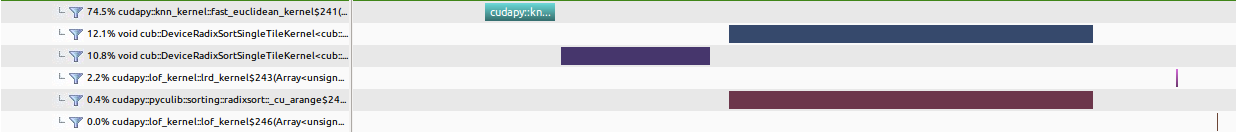
\includegraphics[width=15cm]{Figures/timeline}
\caption{The timeline of all the kernels in GPU}
\label{fig:timeline}
\end{figure}

\subsection{Accuracy}

In measuring of accuracy, I used the \textit{KddCup99} network intrusion detection dataset from UCI machine learning repository\footnote{http://archive.ics.uci.edu/ml/datasets.html} and compare the result of the proposed C\_LOF algorithm with the classical distanced-based algorithm over streaming data (DODDS) where no historical data is considered. The result is measured based on the \textit{F-measure}, which is a widely used method for detecting accuracy of an algorithm. The accuracy of \textit{F-measure} method is decided by F-score, which is defined as:

\[ F_{score} = \frac{2 \times precision \times recall}{precision + recall}  \]

where precision is defined as the number of correctly detected outliers (true positives) divided by the total number of detected outliers (true positives + false positives). Recall is defined as the number of correctly detected outliers divided by the total number of outliers in the dataset (true positives + false negatives). 

The dataset has been split into 10 windows, with each comprises of 1024 data points and is fed to the application one at a time to simulate a streaming environment in a real world. F-score is calculated after all data has been exhausted. The following graph shows the result of evaluation:

\includeFig{fig:f-measure}{Figures/f-measure}{Accuracy comparison between C\_LOF and DODDS}

From the Bar Chart \ref{fig:f-measure}, we see that the C\_LOF algorithm performs only better in the Recall part  but left much to improve in Precision part as well as the overall F-Score. This implies that the C\_LOF generate a large number of false positive results. I think this may be highly related to the choosing of the hyper-parameter $\theta$, which decides the sensitivity of deciding being outlierness. A smaller number of $\theta$ would lead to new data point being classified as outlier easily even if its LOF score deviates little bit from the rest while a larger number of $\theta$ will cause a data point to be hardly classified as outlier and it will only do so if its LOF score deviates far from the rest. Ideally, this hyper-parameter should be adjusted dynamically as more data being observed. 

\subsection{Scalability}

We measure the scalability of the proposed C\_LOF algorithm with respect to the number of data size $N$ and dimension of data point $D$. The result is compared with a CPU sequential implementation of LOF from Python Sklearn library\footnote{http://scikit-learn.org/stable/auto\_examples/neighbors/plot\_lof.html}. The following show the results of these comparisons.

Figure \ref{fig:scalability-D} presents the average time (scaled between 0 and 1) spent on C\_LOF and LOF algorithms respectively to process a random generated dataset with respect to increasing number of attributes (up until 64) over the dataset. We fix the settings on the number of data size N to 1024 and the number of K in K nearest neighbors to 20 before making comparisons. 

\includeFig{fig:scalability-D}{Figures/scalability-D}{Scalability of C\_LOF and LOF with respect to dimension D}
%\includeFig{fig:C_LOF_D}{Figures/C_LOF_D}{Scalability of C\_LOF with respect to dimension D}
%\includeFig{fig:LOF_D}{Figures/LOF_D}{Scalability of LOF with respect to dimension D}

From the graph, we hardly notice any linear increase on the time spent on processing of the data with respect to the increasing of dimension in dataset in C\_LOF algorithm. This implies that we may have not yet made used of every possible resources available in GPU and there are still many rooms to further process even more higher dimension of data. On the other hand, the sequential implementation of LOF seems to scales well so far with respect to data dimension but the overall time spent on processing of data is significantly longer when data dimension become larger compared to C\_LOF. 

Figure \ref{fig:scalability-N} shows how these two algorithms scale with respect to the data size N in logarithmic scale between $[0, 1]$, given a fixed setting of dimension D and KNN size K. We can see that the C\_LOF perform slightly better compared to the sequential implementation over increasing number of data size. 

\includeFig{fig:scalability-N}{Figures/scalability-N}{Scalability of C\_LOF and LOF with respect to data size N}

Due to the limitation on the hardware memory resource in this project, I am not physically capable of processing data with dimension higher than 64, and data size higher than 1024. It will be interesting to see how the runtimes of both implementations will behave on a larger dimension of data and larger data size. 
% ############################################################################
\section{Conclusion} \label{concl}
% ############################################################################

In this project, I implemented a novel extension to the existing LOF algorithm, called C\_LOF using parallel programming techniques including CUDA and MapReduce to detect outliers in a dynamic streaming environment. In doing so, I kept a statistical binned summary based on previous observed data in order to help predict the future outliers. The CUDA framework is used to calculate the LOF scores of each incoming data in GPU while the binned summary is updated using MapReduce programming paradigm. To further accelerate the computation speed in GPU, coalesced memory access is enforced and shared memory is used in order to maximize the bandwidth of data transfer between CPU and GPU. The results of the experiment indeed showed that the proposed method can scale well and generate results faster(little bit) w.r.t the increasing of number in both data size and dimension compared to a sequential implementation. However, the results also suggest that the accuracy of the algorithm, especially the precision part still have much to be improved. And as discussed earlier, this is due to the choosing of the hyper-parameter. A more suitable solution to this problem would be in such a case when deciding the outlierness in the current data stream, we not only consider the historical data, but also consider the future data! This means the algorithm should not report outliers immediately after calculating its LOF scores, but rather treat it as a candidate outlier and only report it as an outlier after observing enough future data points of window size $n$ if it still satisfy the outlier conditions to give more confidence on the results. This can be implemented by assigning a rank to each candidate outliers and increase/decrease its rank after observing a future window. I will leave this to be a future research topic and it would be interesting to see if the accuracy can be improved by using this approach. 

One potential improvement on this project is the implementation of the Kernels on GPUs. Even though we see some improvements in terms of performance compared to the sequential implementation, we did not observe any dramastic speedup(20X). This may due to my in-experience of coding with CUDA and GPU environment as well as resorting to Python's numba complier\footnote{https://numba.pydata.org/} as an implementation of CUDA Kernels. I believe there are many places in the code that can be further optimized by a more experienced CUDA developer as well as writing the code natively in C or C++. Another potential place for speedup is the sorting part, where currently it implements a radix sort using a drop-in CUDA library. Since I did not find any alternative GPU library for sorting, I have to resort to radix sort in this project. Theoretically bitonic sort should be ideal and perform faster better compared to radix sort in a parallel environment. 

% ############################################################################
% Bibliography
% ############################################################################
\bibliographystyle{plain}
\bibliography{my-bibliography}     %loads my-bibliography.bib

% ============================================================================
\end{document}
% ============================================================================
